\documentclass[12pt,a4paper]{article}

\usepackage[a4paper,margin=1in]{geometry}
\usepackage[T1]{fontenc}
\usepackage[utf8]{inputenc}
\usepackage{lmodern}
\usepackage{microtype}
\usepackage{xcolor}
\usepackage{hyperref}
\usepackage{booktabs}
\usepackage{array}
\usepackage{longtable}
\usepackage{enumitem}
\usepackage{listings}
\usepackage{tikz}
\usetikzlibrary{arrows.meta,positioning,shapes.geometric}

\definecolor{primary}{HTML}{1F7A5C}
\definecolor{secondary}{HTML}{2F4858}
\definecolor{lightgray}{HTML}{F5F7F9}
\definecolor{codegray}{HTML}{F8F9FA}
\definecolor{codeborder}{HTML}{D7DEE8}

\hypersetup{
    colorlinks=true,
    linkcolor=primary,
    urlcolor=primary,
    citecolor=primary,
    pdftitle={Technical Report: Viem NFT Marketplace},
    pdfauthor={Project Technical Documentation}
}

\lstdefinestyle{soliditystyle}{
    backgroundcolor=\color{codegray},
    basicstyle=\ttfamily\small,
    breaklines=true,
    frame=single,
    rulecolor=\color{codeborder},
    numbers=left,
    numberstyle=\tiny\color{gray},
    keywordstyle=\color{primary}\bfseries,
    commentstyle=\color{gray},
    stringstyle=\color{secondary},
    showstringspaces=false,
    tabsize=2
}

\setlist[itemize]{leftmargin=1.4em}
\setlist[enumerate]{leftmargin=1.6em}
\renewcommand{\arraystretch}{1.25}

\title{
    \vspace{-1.2cm}
    \textbf{Technical Report}\\
    \large Viem NFT Marketplace
}
\author{NFT Marketplace v2 Project}
\date{May 2026}

\begin{document}

\maketitle

\begin{abstract}
This report documents the design and implementation of \textit{nft-marketplace-v2}, a local NFT marketplace built with Solidity, OpenZeppelin, Hardhat 3, Viem, TypeScript, React, and Vite. The system contains an ERC-721 minting contract, an escrow-based marketplace contract, deployment and demo scripts, automated tests, and a wallet-connected frontend. The marketplace supports NFT minting, token approval, listing creation, price updates, listing cancellation, exact-price purchase execution, seller payouts, and marketplace fee collection.
\end{abstract}

\tableofcontents
\newpage

\section{Introduction}

Non-fungible token marketplaces require coordination between token ownership, marketplace custody, payment settlement, and a user-facing transaction interface. This project implements a compact but complete local marketplace flow for ERC-721 assets. It is designed primarily for development, demonstration, and testing on a local Hardhat network, while also including configuration paths for public test networks such as Sepolia.

The project has three main layers:

\begin{itemize}
    \item \textbf{Smart contracts}: Solidity contracts for ERC-721 minting and marketplace escrow.
    \item \textbf{Blockchain tooling}: Hardhat 3, Viem, deployment scripts, an Ignition module, and tests.
    \item \textbf{Frontend application}: A React and Vite interface for wallet connection, minting, listing, buying, and cancellation.
\end{itemize}

\section{Project Objectives}

The core objectives of the project are:

\begin{enumerate}
    \item Provide a simple ERC-721 token contract with URI-based metadata.
    \item Implement an escrow marketplace where listed NFTs are transferred to the marketplace contract.
    \item Enforce reliable listing state transitions: active, sold, and canceled.
    \item Support marketplace fee calculation in basis points.
    \item Provide a local developer workflow for compile, test, deploy, demo, and frontend use.
    \item Offer a React interface that interacts with the deployed contracts through Viem.
\end{enumerate}

\section{Technology Stack}

\begin{longtable}{p{0.28\linewidth} p{0.64\linewidth}}
\toprule
\textbf{Component} & \textbf{Technology and Purpose} \\
\midrule
\endhead
Smart contracts & Solidity \texttt{0.8.28} with OpenZeppelin contracts for ERC-721, ownership, and reentrancy protection. \\
Contract framework & Hardhat 3 with \texttt{@nomicfoundation/hardhat-toolbox-viem}. \\
Blockchain client & Viem for deployments, tests, frontend reads, wallet writes, and ETH formatting/parsing. \\
Frontend & React 19, TypeScript, Vite, Lucide icons, Motion, and lightweight local UI components. \\
Testing & Node test runner through Hardhat with Viem wallet clients and public client reads. \\
Deployment & Hardhat scripts and an Ignition module. The local deployment script writes addresses into \texttt{src/deployment.ts}. \\
\bottomrule
\end{longtable}

\section{Repository Structure}

\begin{longtable}{p{0.30\linewidth} p{0.62\linewidth}}
\toprule
\textbf{Path} & \textbf{Responsibility} \\
\midrule
\endhead
\texttt{contracts/MyNFT.sol} & ERC-721 minting contract with token URI storage. \\
\texttt{contracts/NFTMarketplace.sol} & Marketplace contract that escrows tokens, tracks listings, processes purchases, and handles fees. \\
\texttt{test/NFTMarketplace.ts} & Automated test suite for minting, listing, updating, cancellation, purchase settlement, access control, and invalid actions. \\
\texttt{scripts/deploy.ts} & Local deployment script that deploys both contracts and updates frontend addresses. \\
\texttt{scripts/demo-marketplace.ts} & End-to-end demo script that deploys, mints, approves, lists, purchases, and prints the final owner. \\
\texttt{ignition/modules/NFTMarketplace.ts} & Hardhat Ignition deployment module with fee recipient and fee basis point parameters. \\
\texttt{src/App.tsx} & Main React application implementing wallet connection and marketplace workflows. \\
\texttt{src/abi.ts} & Contract ABI bindings used by the frontend. \\
\texttt{src/deployment.ts} & Current frontend deployment target: chain ID and contract addresses. \\
\bottomrule
\end{longtable}

\section{System Architecture}

The marketplace follows a contract-centric architecture. The frontend does not maintain authoritative listing state. Instead, it reads listing data from the marketplace contract, resolves token metadata from token URIs, and submits signed transactions through the connected wallet.

\begin{figure}[h]
\centering
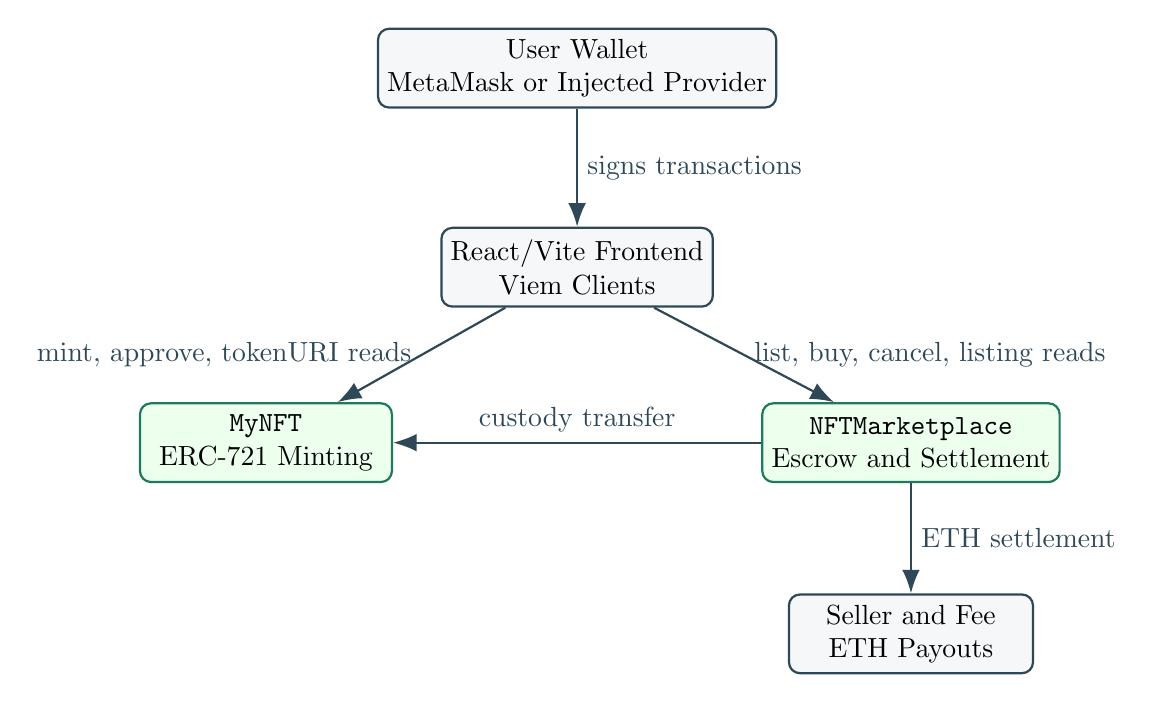
\begin{tikzpicture}[
    node distance=1.5cm,
    box/.style={rectangle, rounded corners, draw=secondary, thick, fill=lightgray, minimum width=3.1cm, minimum height=1cm, align=center},
    contract/.style={rectangle, rounded corners, draw=primary, thick, fill=green!7, minimum width=3.2cm, minimum height=1cm, align=center},
    arrow/.style={-{Latex[length=3mm]}, thick, color=secondary}
]
    \node[box] (user) {User Wallet\\MetaMask or Injected Provider};
    \node[box, below=of user] (frontend) {React/Vite Frontend\\Viem Clients};
    \node[contract, below left=1.2cm and 0.6cm of frontend] (nft) {\texttt{MyNFT}\\ERC-721 Minting};
    \node[contract, below right=1.2cm and 0.6cm of frontend] (market) {\texttt{NFTMarketplace}\\Escrow and Settlement};
    \node[box, below=1.4cm of market] (seller) {Seller and Fee\\ETH Payouts};

    \draw[arrow] (user) -- node[right]{signs transactions} (frontend);
    \draw[arrow] (frontend) -- node[left]{mint, approve, tokenURI reads} (nft);
    \draw[arrow] (frontend) -- node[right]{list, buy, cancel, listing reads} (market);
    \draw[arrow] (market) -- node[above]{custody transfer} (nft);
    \draw[arrow] (market) -- node[right]{ETH settlement} (seller);
\end{tikzpicture}
\caption{High-level architecture of the NFT marketplace.}
\end{figure}

\section{Smart Contract Design}

\subsection{MyNFT Contract}

\texttt{MyNFT} extends OpenZeppelin's \texttt{ERC721URIStorage}. It defines the collection name \textit{Viem Marketplace NFT} and symbol \textit{VMNFT}. The contract tracks the total number of minted tokens through \texttt{totalMinted}.

The contract provides two minting entry points:

\begin{itemize}
    \item \texttt{mint(string tokenURI)} mints a token to the caller.
    \item \texttt{mintTo(address to, string tokenURI)} mints a token to a specified recipient.
\end{itemize}

The minting process increments \texttt{totalMinted}, safely mints the token, stores the token URI, and emits a \texttt{TokenMinted} event. The contract rejects minting to the zero address through a custom \texttt{InvalidRecipient} error.

\subsection{NFTMarketplace Contract}

\texttt{NFTMarketplace} implements the main exchange logic. It inherits:

\begin{itemize}
    \item \texttt{IERC721Receiver}, allowing the contract to receive ERC-721 tokens through safe transfers.
    \item \texttt{Ownable}, allowing administrative control over fee settings.
    \item \texttt{ReentrancyGuard}, protecting state-changing listing and purchase flows from reentrant calls.
\end{itemize}

The marketplace stores listings in a mapping from listing ID to a \texttt{Listing} struct. It also maintains \texttt{listingByToken}, which maps an NFT contract and token ID to its active listing ID.

\begin{lstlisting}[style=soliditystyle, language=Java, caption={Listing data model used by the marketplace contract.}]
enum ListingStatus {
    None,
    Active,
    Sold,
    Canceled
}

struct Listing {
    uint256 listingId;
    address nft;
    uint256 tokenId;
    address payable seller;
    uint256 price;
    ListingStatus status;
    address buyer;
}
\end{lstlisting}

\subsection{Listing Lifecycle}

The listing lifecycle is intentionally small and auditable:

\begin{enumerate}
    \item The seller owns an ERC-721 token.
    \item The seller approves the marketplace for that token.
    \item The seller calls \texttt{createListing}.
    \item The marketplace verifies ownership, records the listing, and escrows the NFT.
    \item The seller may update the price or cancel the listing while it is active.
    \item A buyer purchases the listing by sending exactly the listing price.
    \item The marketplace transfers the NFT to the buyer and splits ETH between the seller and fee recipient.
\end{enumerate}

\subsection{Fee Model}

Marketplace fees are represented in basis points. The denominator is \texttt{10,000}, so a fee of \texttt{250} basis points equals \texttt{2.5\%}. The contract caps marketplace fees at \texttt{1,000} basis points, or \texttt{10\%}, through \texttt{MAX\_MARKETPLACE\_FEE\_BPS}.

For a listing price \(P\) and fee \(F_{bps}\), the fee is calculated as:

\[
    \text{marketplaceFee} = \frac{P \times F_{bps}}{10000}
\]

The seller receives:

\[
    \text{sellerProceeds} = P - \text{marketplaceFee}
\]

\subsection{Administrative Controls}

The owner can update:

\begin{itemize}
    \item \texttt{marketplaceFeeBps}, subject to the maximum fee cap.
    \item \texttt{feeRecipient}, subject to a non-zero address requirement.
\end{itemize}

Both administrative actions emit events, which makes off-chain indexing and monitoring easier.

\section{Frontend Design}

The frontend is implemented in \texttt{src/App.tsx}. It uses Viem to create:

\begin{itemize}
    \item A \texttt{publicClient} for read-only contract calls and transaction receipt waiting.
    \item A wallet client using \texttt{custom(window.ethereum)} for signed transactions.
\end{itemize}

\subsection{Main User Workflows}

The interface supports the following workflows:

\begin{enumerate}
    \item \textbf{Connect wallet}: Requests wallet accounts and switches to the configured marketplace chain.
    \item \textbf{Mint NFT}: Calls \texttt{MyNFT.mint}, then reads \texttt{totalMinted} to prefill the token ID for listing.
    \item \textbf{Approve and list}: Approves the marketplace for a token and then calls \texttt{createListing}.
    \item \textbf{Browse listings}: Reads all listing IDs from \texttt{1} to \texttt{listingCount}, filters active listings, and resolves metadata.
    \item \textbf{Buy listing}: Calls \texttt{purchaseListing} with the exact listing price as transaction value.
    \item \textbf{Cancel own listing}: Calls \texttt{cancelListing} for listings where the connected account is the seller.
\end{enumerate}

\subsection{Metadata Handling}

The frontend reads \texttt{tokenURI} from \texttt{MyNFT}. It handles direct image URLs and JSON metadata URLs. It also converts \texttt{ipfs://} URIs to the public \texttt{https://ipfs.io/ipfs/} gateway. Metadata fetches have a timeout, and missing metadata falls back to a token-number label.

\subsection{Market Navigation}

The UI includes search, filtering, sorting, market statistics, and listing cards. Listings can be filtered by all listings, listings owned by the connected wallet, and listings available for purchase. Sorting supports newest first, low price first, and high price first.

\section{Deployment and Local Operation}

The recommended local workflow is:

\begin{enumerate}
    \item Install dependencies with \texttt{npm install}.
    \item Start a Hardhat node with \texttt{npm run node}.
    \item Deploy contracts with \texttt{npm run deploy}.
    \item Start the frontend with \texttt{npm run dev}.
    \item Connect a wallet to chain \texttt{31337}.
\end{enumerate}

The deployment script deploys \texttt{MyNFT} first, then deploys \texttt{NFTMarketplace} with the fee recipient and default fee of \texttt{250} basis points. It then writes the frontend deployment configuration to \texttt{src/deployment.ts}. At the time of inspection, the local deployment configuration targets chain \texttt{31337}.

\section{Security Considerations}

The project applies several important smart contract safety practices:

\begin{itemize}
    \item \textbf{Escrow custody}: Listed NFTs are held by the marketplace, preventing sellers from transferring listed assets away before purchase.
    \item \textbf{Exact payment enforcement}: Purchases require \texttt{msg.value == listing.price}, avoiding ambiguous overpayment or underpayment behavior.
    \item \textbf{Reentrancy protection}: Listing creation, cancellation, and purchase are protected with \texttt{nonReentrant}.
    \item \textbf{Checks-effects-interactions structure}: Purchase state is updated before NFT and ETH transfers.
    \item \textbf{Custom errors}: The contracts use explicit custom errors for invalid addresses, zero prices, inactive listings, unauthorized sellers, self-purchases, and failed payouts.
    \item \textbf{Fee cap}: The owner cannot set the marketplace fee above \texttt{10\%}.
\end{itemize}

Some limitations remain appropriate for a local demonstration project:

\begin{itemize}
    \item The marketplace currently supports fixed-price listings only.
    \item Listing discovery in the frontend scans from \texttt{1} to \texttt{listingCount}, which is simple but not suitable for very large markets.
    \item The NFT contract has open minting and does not restrict who can mint.
    \item The marketplace does not implement royalties such as ERC-2981.
    \item ETH payouts use direct calls; failed seller or fee-recipient payouts revert the full purchase.
\end{itemize}

\section{Testing and Verification}

The project includes a focused automated test suite in \texttt{test/NFTMarketplace.ts}. The tests cover:

\begin{itemize}
    \item NFT minting and token URI storage.
    \item Listing creation and escrow transfer.
    \item Listing price updates by the seller.
    \item Listing cancellation and NFT return.
    \item Purchase execution, buyer ownership transfer, seller proceeds, and fee recipient payment.
    \item Rejection of invalid listing and purchase actions.
    \item Owner-only marketplace fee and recipient configuration.
\end{itemize}

\subsection{Verification Results}

The following commands were run successfully:

\begin{longtable}{p{0.30\linewidth} p{0.54\linewidth} p{0.10\linewidth}}
\toprule
\textbf{Command} & \textbf{Result} & \textbf{Status} \\
\midrule
\endhead
\texttt{npm test} & Hardhat test suite completed with \texttt{7 passing}. & Pass \\
\texttt{npm run typecheck} & TypeScript compiler completed with no reported errors. & Pass \\
\texttt{npm run build} & Hardhat compile completed and Vite produced a production build in \texttt{dist/}. & Pass \\
\bottomrule
\end{longtable}

The production build emitted a Vite chunk-size warning for a generated JavaScript asset above 500 kB. This is not a build failure, but future optimization could introduce dynamic imports or manual Rollup chunks.

\section{End-to-End Marketplace Flow}

The demo script \texttt{scripts/demo-marketplace.ts} executes the complete marketplace flow on an in-memory Hardhat network:

\begin{enumerate}
    \item Deploy \texttt{MyNFT} and \texttt{NFTMarketplace}.
    \item Mint a token to the seller.
    \item Approve the marketplace to transfer the token.
    \item Create a listing for \texttt{0.25 ETH}.
    \item Purchase the listing from a buyer account.
    \item Read and print the new token owner.
\end{enumerate}

This script is useful as a quick sanity check because it validates the main interaction path without requiring a browser wallet.

\section{Potential Enhancements}

The following improvements would make the project more production-like:

\begin{itemize}
    \item Add event indexing or a subgraph-style data layer for scalable listing discovery.
    \item Add support for ERC-2981 royalties.
    \item Add bid, auction, or collection offer functionality.
    \item Add pagination and event-based refreshes to the frontend.
    \item Add wallet balance display and clearer chain mismatch handling.
    \item Add deployment configuration for multiple networks without overwriting local frontend addresses.
    \item Add static analysis tooling such as Slither and contract coverage reporting.
    \item Split frontend bundles if production size becomes important.
\end{itemize}

\section{Conclusion}

\textit{nft-marketplace-v2} is a complete local NFT marketplace implementation with clear separation between token minting, marketplace settlement, deployment tooling, testing, and frontend interaction. The smart contract design uses escrow custody, explicit state transitions, fee-capped basis point accounting, and reentrancy protection. The React frontend provides the expected marketplace workflows and uses Viem consistently for both read and write operations. Automated tests and build verification passed, making the project a solid foundation for further marketplace features, indexing, royalties, or public testnet deployment.

\end{document}
